\documentclass[9pt,twocolumn,twoside]{styles/osajnl}
\usepackage{fancyvrb}
\journal{i524} 

\title{Twister: A new approach to MapReduce Programming}


\author[1,*]{Vasanth Methkupalli}

\affil[1]{School of Informatics and Computing, Bloomington, IN 47408, U.S.A.}


\affil[*]{Corresponding authors: mvasanthiiit@gmail.com}

\dates{Paper-1, \today}

\ociscodes{MapReduce, Twister, Iterative, reduction, combine}

% replace this with your url in github/gitlab
\doi{\url{https://github.com/cloudmesh/sp17-i524/blob/master/paper1/S17-IR-2019/report.pdf}}


\begin{abstract}
MapReduce is a method to process vast sums of data in parallel without
requiring the developer to write any other code other than the mapper
and reduce functions.  Starting with Google in 2004 there has been a
lot of research going on in this particular field since the rate at
which data is increasing is exponential. The need to store the data
and analyze has become of paramount importance in the current
situation. This has lead the researcher's to look for various parallel
processing programming models to saturate the needs. Of these MPI,
MapReduce are some of the examples which has produced good results to
the scientific community. Here in this paper we examine an
implementation of MapReduce programming model, Twister, which exhibits
some improvements over the current model.
\newline
\end{abstract}

\setboolean{displaycopyright}{true}

\begin{document}

\maketitle

\section{Introduction}

Emergence of massive data sets in many areas and settings have
presented many challenges and opportunities in data storage and
analysis\cite{dean2008mapreduce}\cite{mohebi2016iterative}. Traditional
analytic tools many a times cannot live up to the needs and demands at
the ongoing rate at which data is produced to store and analyze
it\cite{lee2012parallel}. However, domain knowledge and research have
given rise to new tools and technologies which has made many of these
tasks easier\cite{zaharia2010spark}. Google’s MapReduce falls in to
one of these categories. The MapReduce programming framework uses two
tasks common in functional programming: Map and Reduce, Map()
procedure (method) that performs filtering and sorting, Reduce()
method that performs a summary operation(merging the
results)\cite{wikipedia}\cite{mohammed2014applications}. MapReduce is
a new parallel processing framework and Hadoop is its open-source
implementation on a single computing node or on clusters. Compared
with existing parallel processing paradigms (e.g. grid computing and
graphical processing unit (GPU)), MapReduce and Hadoop have two
advantages:1) Fault-tolerant storage resulting in reliable data
processing by replicating the computing tasks, and cloning the data
chunks on different computing nodes across the computing cluster. 2)
High-throughput data processing via a batch processing framework and
the Hadoop distributed file system
(HDFS)\cite{elsayed2014mapreduce}\cite{ekanayake2010twister}\cite{lee2012parallel}.


Data are stored in the HDFS and made available to the slave nodes for
computation. A MapReduce program consists of the "MapReduce System"
(also called "infrastructure" or "framework") orchestrates the
processing by marshalling the distributed servers, running the various
tasks in parallel, managing all communications and data transfers
between the various parts of the system, and providing for redundancy
and fault tolerance\cite{mohammed2014applications}. MapReduce
programming model has simplified the implementations of many data
parallel applications\cite{lee2012parallel}. The simplicity of the
programming model and the quality of services provided by many
implementations of MapReduce attract a lot of enthusiasm among
parallel computing
communities\cite{ekanayake2010twister}\cite{grolinger2014challenges}. It
has been identified that MapReduce can be extended to many other
applications by improving on the programming model and the
architecture. In this regard, Twister attempts to extend the Google’s
MapReduce application to more class of applications by including more
features\cite{twister}\cite{doulkeridis2014survey}.




\begin{figure}[htbp]
\centering
\fbox{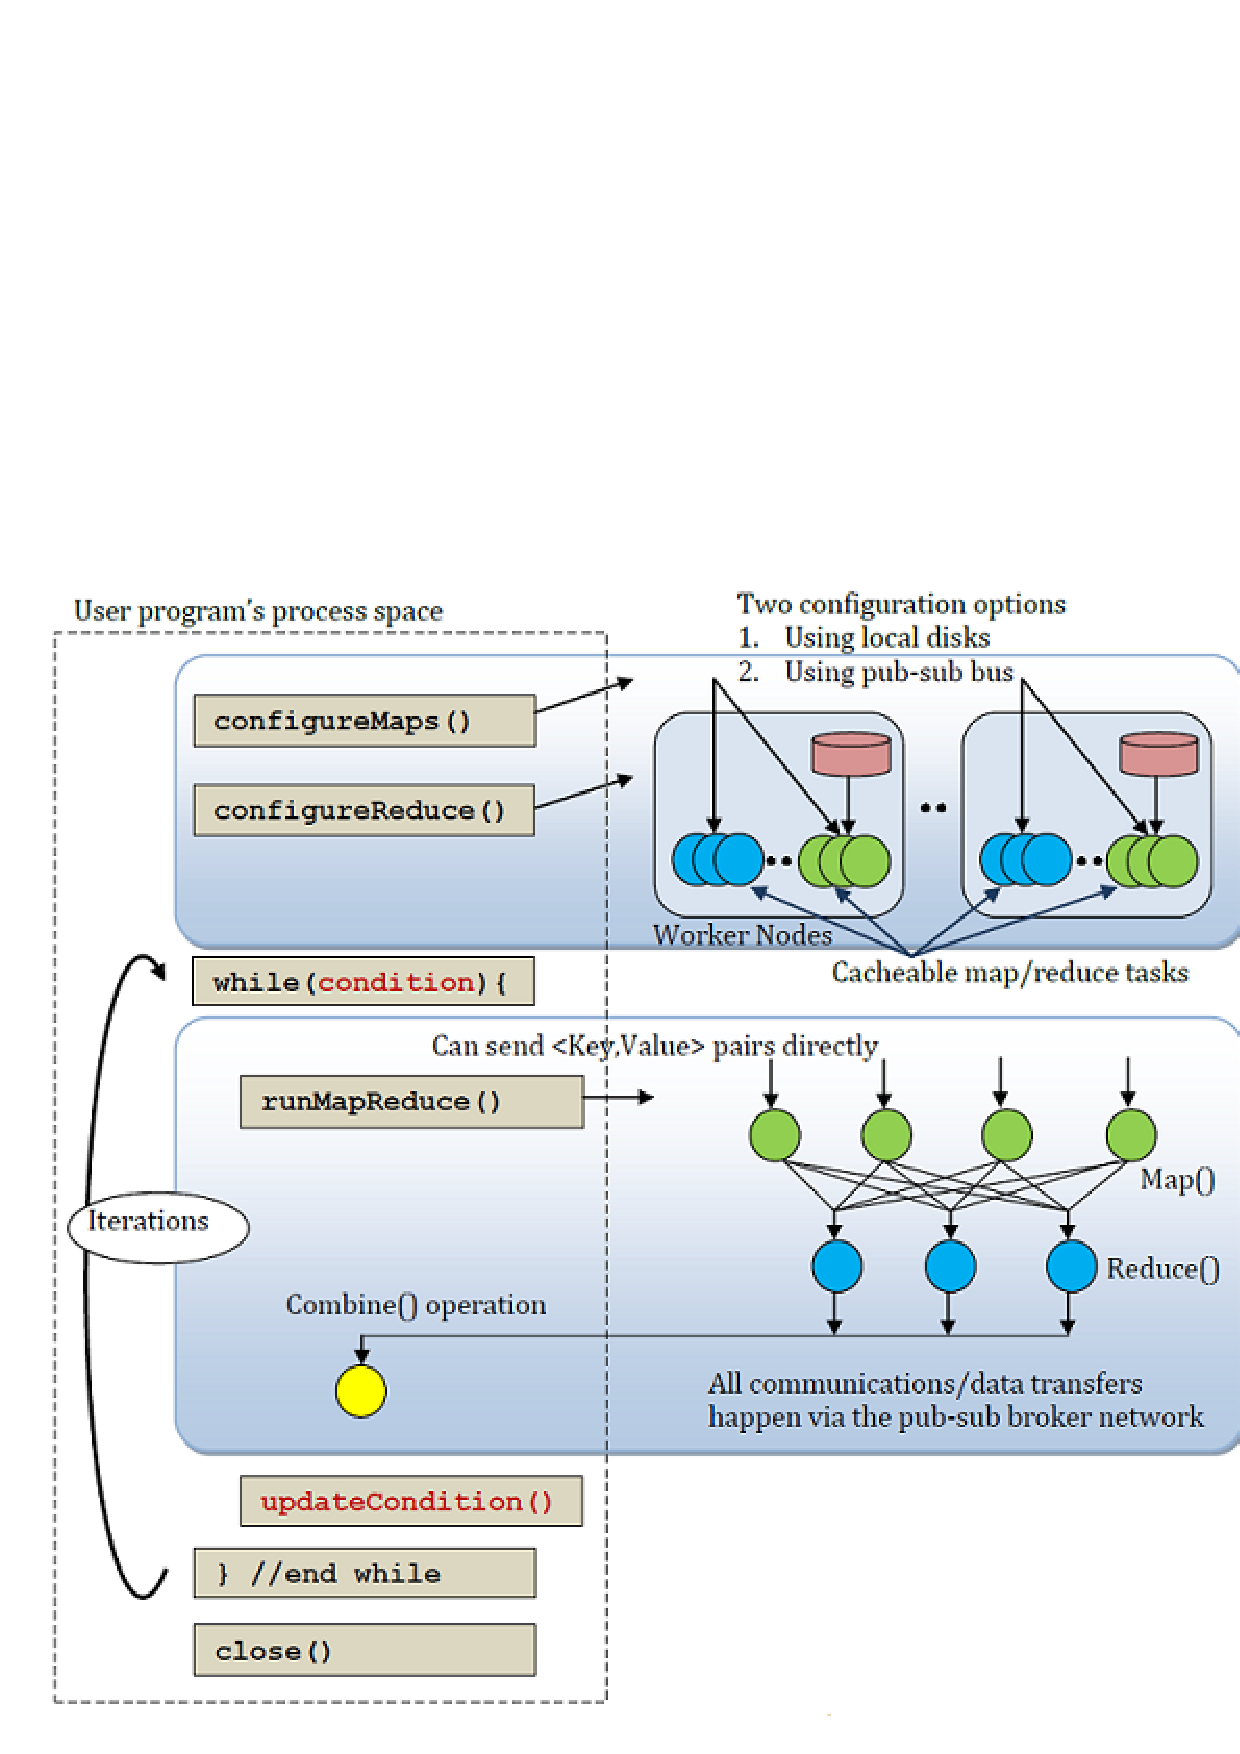
\includegraphics[width=\linewidth]{images/a}}
\caption{Twister Programming model.}
\label{fig:Twister Programming model}
\end{figure}


\section{Twister:}

Twister was developed as a part of Ph.D. research and is an going
research project by the SALSA team
@IU\cite{grolinger2014challenges}\cite{dean2008mapreduce}. Identifying
many problems in MapReduce programming model, they have envisioned to
develop a better version to apply it to various scientific
applications\cite{zaharia2010spark}. A set of extensions to the
programming model and improvements to its architecture that will
expand the applicability of MapReduce to more classes of
applications\cite{elsayed2014mapreduce}. Twister is a lightweight
MapReduce runtime that has been developed by incorporating these
enhancements\cite{ekanayake2010twister}\cite{lee2012parallel}. Twister
provides the following features to support MapReduce computations. 1)
Distinction on static and variable data 2) Configurable long running
(cacheable) map/reduce tasks 3) Pub/sub messaging based
communication/data transfers 4) Efficient support for Iterative
MapReduce computations (extremely faster than Hadoop or
Dryad/DryadLINQ) 5) Combine phase to collect all reduce outputs 6)
Data access via local disks 7) Lightweight (~5600 lines of Java code)
8) Support for typical MapReduce computations 9) Tools to manage
data\cite{twister}\cite{doulkeridis2014survey}.





\section{Twister improvements over MapReduce programming model:}
\label{sec:examples}


\subsection{Static vs. Dynamic Data}
In all the iterative applications which were observed, they showed two
types of data formats, one-static data, two-dynamic data\cite{grolinger2014challenges}.  Static data
is data which is fixed throughout the computation whereas the variable
data(Dynamic Data) is the computed results in each iteration and
typically consumed in the next iteration in other applications, one of
which example is an expectation minimization algorithms\cite{doulkeridis2014survey}.

\subsection{Canceable Mappers/Reducers}
Although some of the typical MapReduce computations such as
distributed sorting and information retrieval consume very large data
sets, many iterative applications we encounter operate on moderately
sized data sets which can fit into the distributed memory of the
computation clusters\cite{elsayed2014mapreduce}. This observation led
us to explore the idea of using long running map/reduce tasks similar
to the long running parallel processes in many MPI applications which
last throughout the life of the computation. The long running
(cacheable) map/reduce tasks allow map/reduce tasks to be configured
with static data and use them without loading again and again in each
iteration\cite{lee2012parallel}. Current MapReduce implementations
such as Hadoop and DryadLINQ do not support this behavior and hence
they initiate new map/reduce tasks and load static data in each
iteration incurring considerable performance overheads\cite{twister}.

\subsection{Supports "side-effect-free" Programming}
Twister has long running map-reduce takes by which it does not
encourage users to store state information in the map/reduce
tasks. Thereby, achieving the side-effect-free nature of
MapReduce. Caching the static data across map/reduce tasks helps in
achieving better thoroughput\cite{lee2012parallel}. This framework
does not ensure the use of same set of map/reduce tasks throughout the
life of an iterative computation\cite{twister}.

\subsection{Combine Step as Further Reduction}
Twister also introduce an optional reduction phase named "combine",
which is another reduction phase that can be used to combine the
results of the reduce phase into a single value. The user program and
the combine operation run on a single process space allowing its
output directly accessible to the user
program\cite{grolinger2014challenges}. This enables the user to check
conditions based on the output of the MapReduce
computations\cite{twister}.

\subsection{Uses Pub/sub messaging}
Twister uses pub/sub messaging for all the communication/data transfer
requirements which eliminates the overhead in transferring data via
file systems as in Hadoop orDryadLINQ\cite{grolinger2014challenges}. The output <Key,Value> pairs
produced during the map stage get transferred directly to the reduce
stage and the output of the reduce stage get transferred directly to
the combined stage via the pub-sub broker
network\cite{lee2012parallel}. Currently Twister uses
publish-subscribe messaging capabilities of NaradaBrokering messaging
infrastructure, but the framework is extensible to support any other
publish-subscribe messaging infrastructure such as Active MQ
\cite{twister}.

\subsection{Data Access via local disks}
Two mechanisms about data access have been proposed in Twister; (i)
Directly from the local disk of computer nodes, (ii) Directly from the
pub-sub infrastructure\cite{elsayed2014mapreduce}. For the simplicity
of the implementation, Twister provided a file based data access
mechanism for the map/reduce tasks. Unlike Hadoop, twister does not
come with the built in file system. Instead it provides a tool to
manage the data across these distributed disks.  Apart from the above
the use of streaming enables Twister to support features such as
directly sending input <Key,Value> pairs for the map stage from the
user program and configuring map/reduce stages using the data sent
from the user program\cite{mohammed2014applications}.

\subsection{Fault Tolerance}
Providing fault tolerance support for iterative computations with
Twister is currently under development.

\section{Application of Twister to present problems:}

\subsection{K-Means Clustering}
Kmeans clustering is a well-known clustering algorithm aiming to
cluster a set of data points to a predefined number of clusters. In
that each map function gets a portion of the data, and it needs to
access this data split in each iteration. These data items do not
change over the iterations, and it is loaded once for the entire set
of iterations. The variable data is the current cluster centers
calculated during the previous iteration and hence used as the input
value for the map function\cite{twister}\cite{dean2008mapreduce}.

All the map functions get this same input data (current cluster
centers) at each iteration and computes a partial cluster centers by
going through its data set. A reduce function computes the average of
the partial cluster centers and produce the cluster centers for the
next step. Main program, once it gets these new cluster centers,
calculates the difference between the new cluster centers and the
previous cluster centers and determine if it needs to execute another
cycle of MapReduce
computation\cite{ekanayake2008mapreduce}\cite{twister}.


\subsection{Matrix Multiplication}
Let A and B, produce matrix C, as the result of the multiplication
process. Here they split the matrix B into a set of column blocks and
the matrix A into a set of row blocks. In each iteration, all the map
tasks process two inputs: (i) a column block of matrix B, and (ii) a
row block of matrix A; collectively, they produce a row block of the
resultant matrix C. The column block associated with a particular map
task is fixed throughout the computation, while the row blocks are
changed in each iteration. However, in Hadoop's programming model (a
typical MapReduce model), there is no way to specify this behavior.
Hence, it loads both the column block and the row block in each
iteration of the computation. Twister supports the notion of long
running map/reduce tasks where these tasks are allowed to retain
static data in the memory across invocations, yielding better
performance for "Iterative MapReduce"
computations\cite{dean2008mapreduce}\cite{twister}.

\subsection{Page Rank}

In Twister implementation of PageRank, we constructed web graphs with
vertices where in-link degree of all pages comply with the power law
distribution. These input data are partitioned into few parts and
stored in the format of adjacency list. Each map function runs on one
of the partitioned data, which are constant over the iterations. The
variable data are the PageRank values calculated during previous
iteration which in turns used as the input value for the next
iteration. In each iteration, the MAP task updates the old PageRank
values to new one by analyzing the local partial adjacency list
file. The output of MAP task is partial of PageRank values. The reduce
task receives all the partial output and produces the new PageRank
values\cite{twister}.


\subsection{Graph Search}
This algorithm tries to use Twister Framework to process breadth-first
graph search problem in parallel. This algorithm is based on Cailin's
Hadoop version of breadth-first graph search[10]. The basic idea of
this algorithm is to exploring the nodes of the same level parallel,
and then explore the next levels iteratively\cite{twister}.


\subsection{Word Count}

In typical word count applications implemented using other MapReduce
runtimes, the map task outputs (word,1) pairs for all the words it
encounter. This approach is not optimized for performance rather
simple to program. With small amount of more complexity we can simply
convert this map task to produce a list of (word,count) pairs
corresponding to the local data partion. This is the approach used in
Twister word count application\cite{twister}.


\subsection{High Energy Physics(HEP) Data Analysis}

The goal of the analysis is to execute a set of analysis functions on
a collection of data files produced by high-energy physics
experiments. After processing each data file, the analysis produces a
histogram of identified features. These histograms are then combined
to produce the final result of the overall analysis. This data
analysis task is both data and compute intensive and fits very well
for MapReduce computation model. First figure shows the program flow
of this analysis once it is converted to a MapReduce implementation
and the second figure compares the performance of Twister and Hadoop
for this data analysis[12]\cite{twister}.



\section{Conclusion}
It has been observed that changes in the programming model and the way
the nodes interact with each other(pub-sub
messaging)\cite{ekanayake2010twister}, has produced very good results
with Twister MapReduce. This has in turn lead it benificial to many
applications of which many have been discussed in the present
paper. So it can be safe to assume that Twister has a very high scope
for commercial applications even thought it is limited to scientific
applications as of now.


\bibliography{references} 



\end{document}
